\clearpage
\section{Supplementary Material for DONUT}
\label{sec:suppl_topogen}


This section first provides an in-depth analysis of the EuLearn dataset~\cite{eulearn}, to justify why it's not reliable for our experiments. Then, it details the algorithms and proofs related to the DONUT dataset generation process.

\subsection{EuLearn Dataset Analysis}
\label{ssec:suppl_eulearn_analysis}

A key issue is the entanglement between topology and orientation. As shown in Figure~\ref{fig:eulearn-acc-angle}, a simple $k$-nearest neighbor classifier trained on point clouds in their canonical orientation achieves near-perfect accuracy. However, accuracy collapses when test samples are randomly rotated, despite genus being a topological invariant. This indicates that classifiers exploit orientation-dependent cues instead of genuine topological structure.


The same effect appears at the representation level. Figure~\ref{fig:eulearn-umap-comparison} shows UMAP projections of Point-BERT embeddings. When evaluated on canonical orientations, embeddings form tight clusters by genus. After applying random rotations, this structure disappears entirely. If embeddings reflected topology, genus separation should persist under rigid transformations; instead, the disappearance of clusters confirms that the genus signal in EuLearn is largely a proxy for global pose and correlated geometric features.

\begin{figure}[h]
  \centering
  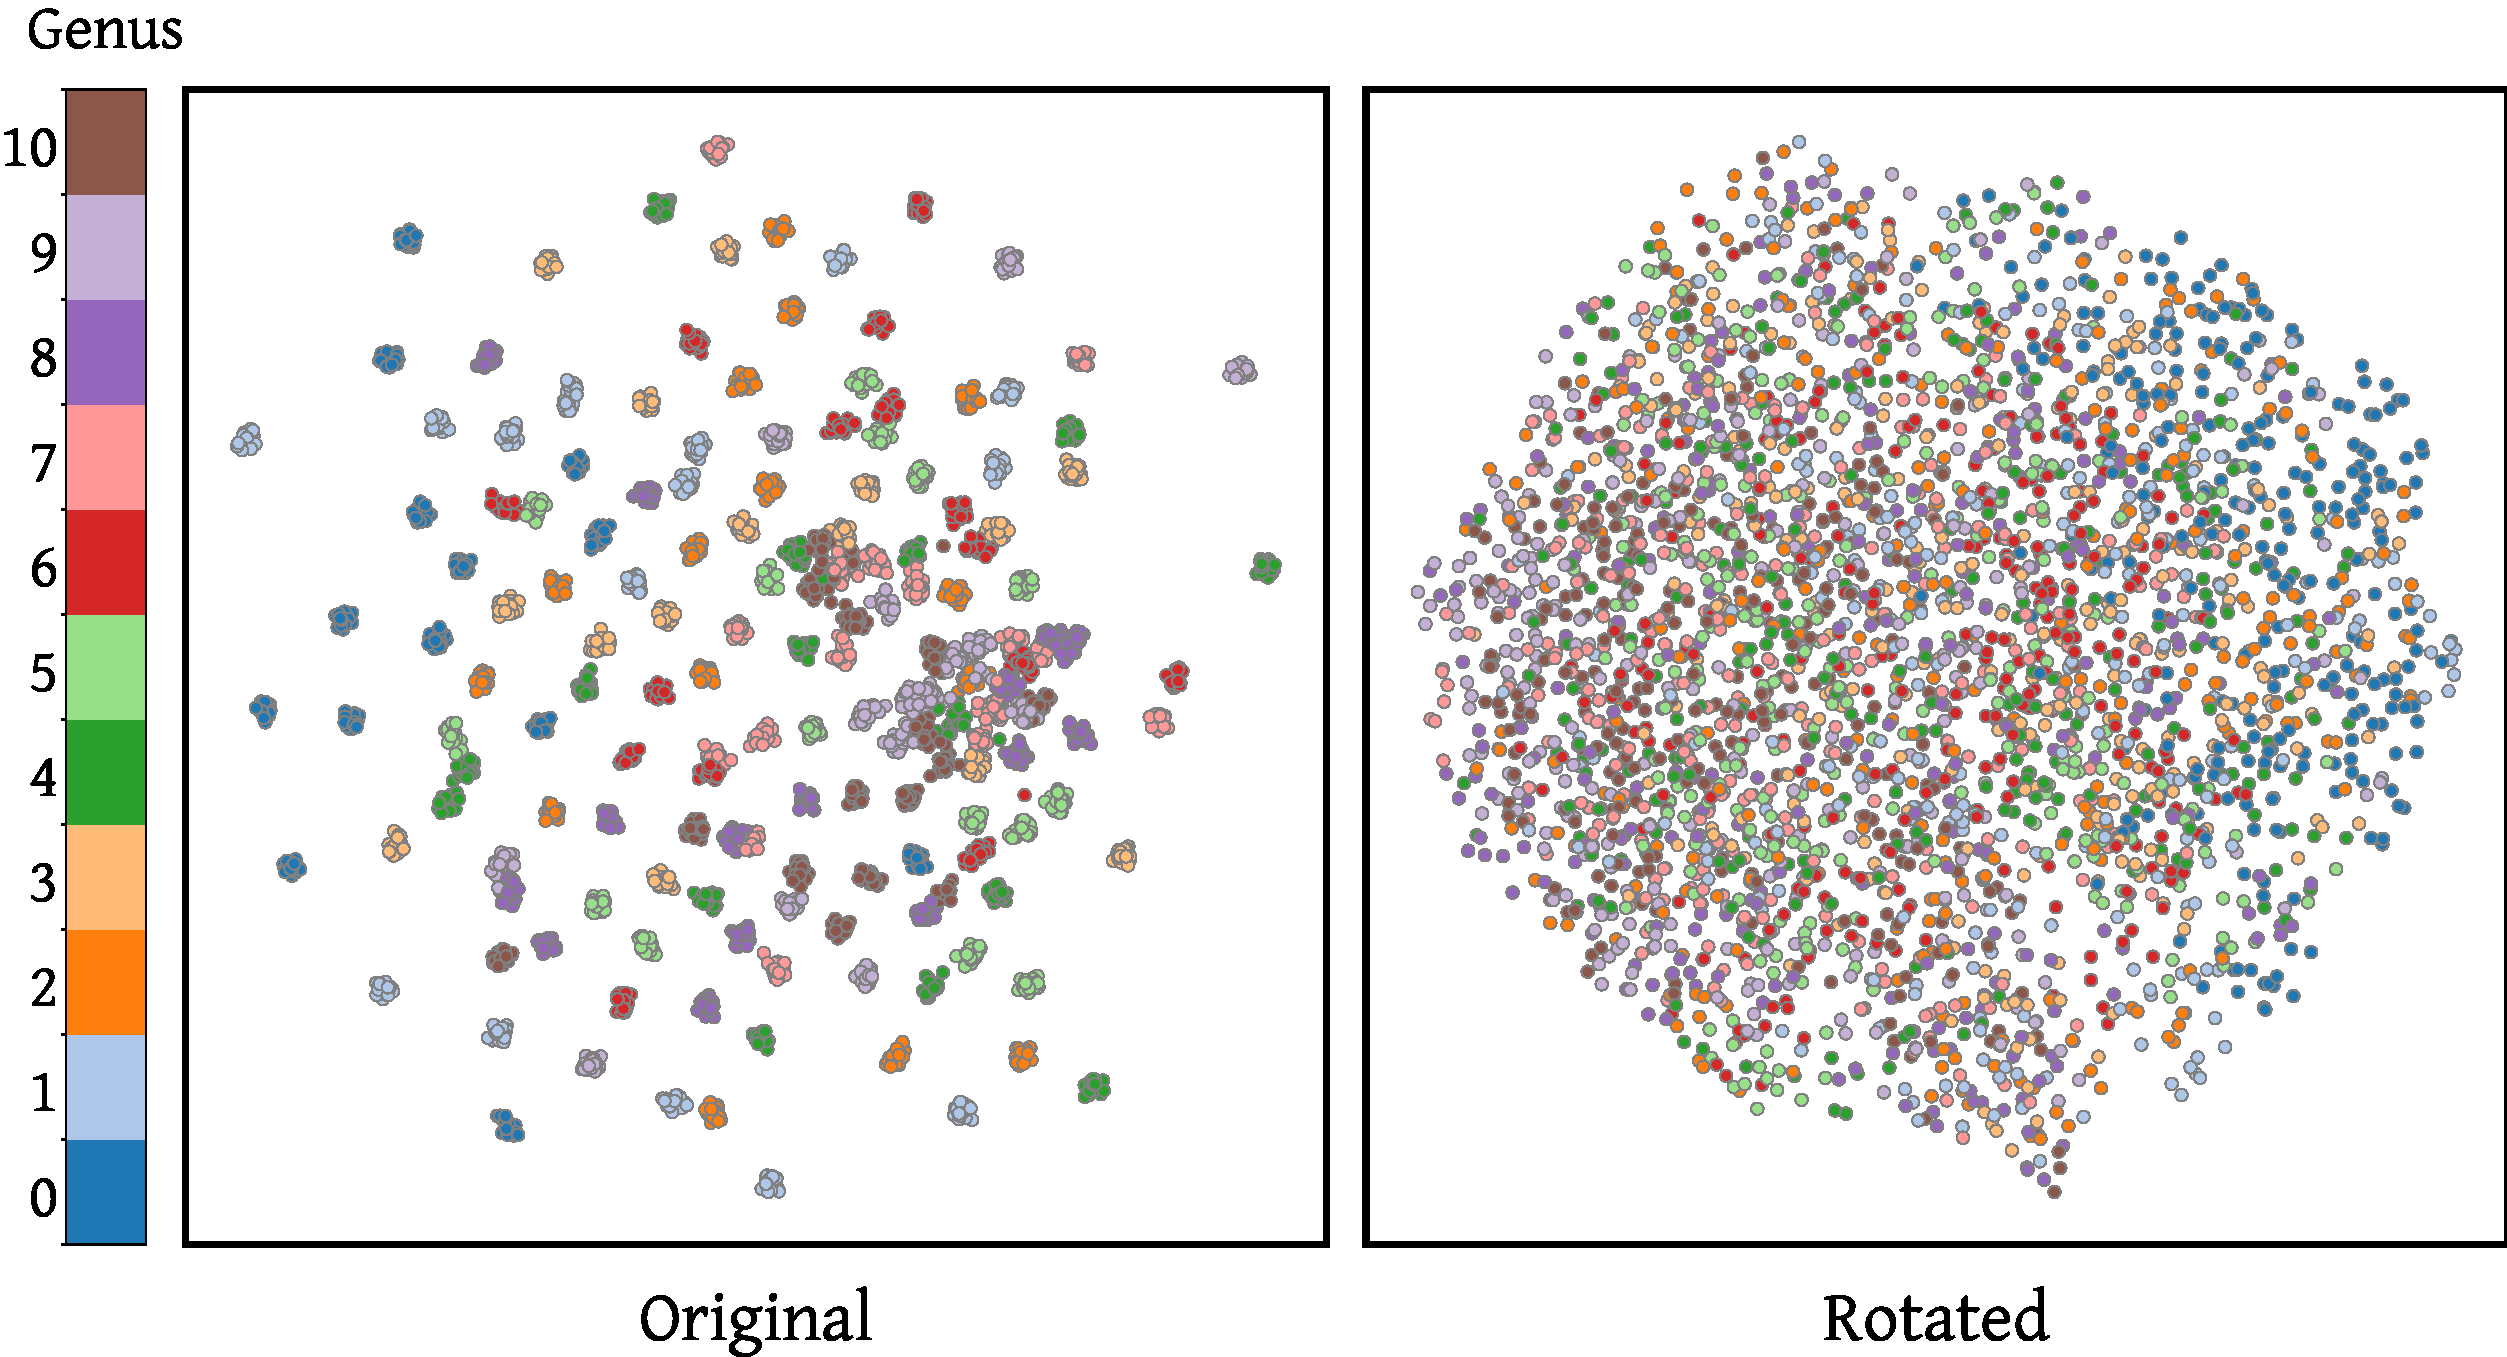
\includegraphics[width=0.7\linewidth]{figs/eulearn/umap_comparison_original_rotated.pdf}
   \caption{\textbf{UMAP projections of Point-BERT embeddings colored by genus.} Clear clusters by genus appear for canonical orientations (left) but vanish under random rotations (right), showing that genus separation in EuLearn is tied to orientation rather than topology.}
   \label{fig:eulearn-umap-comparison}
\end{figure}

Linear probing experiments further reinforce this point (Table~\ref{tab:eulearn-overfit}). Probes trained on canonical embeddings generalize only to canonical test shapes, collapsing under rotations. Probes trained on rotated embeddings avoid orientation bias but fail to recover meaningful genus structure, with accuracies barely above random chance. In both cases, the embeddings overfit to spurious correlations, not topology.

\begin{figure}[h]
\centering
\begin{minipage}{0.45\linewidth}
    \centering
    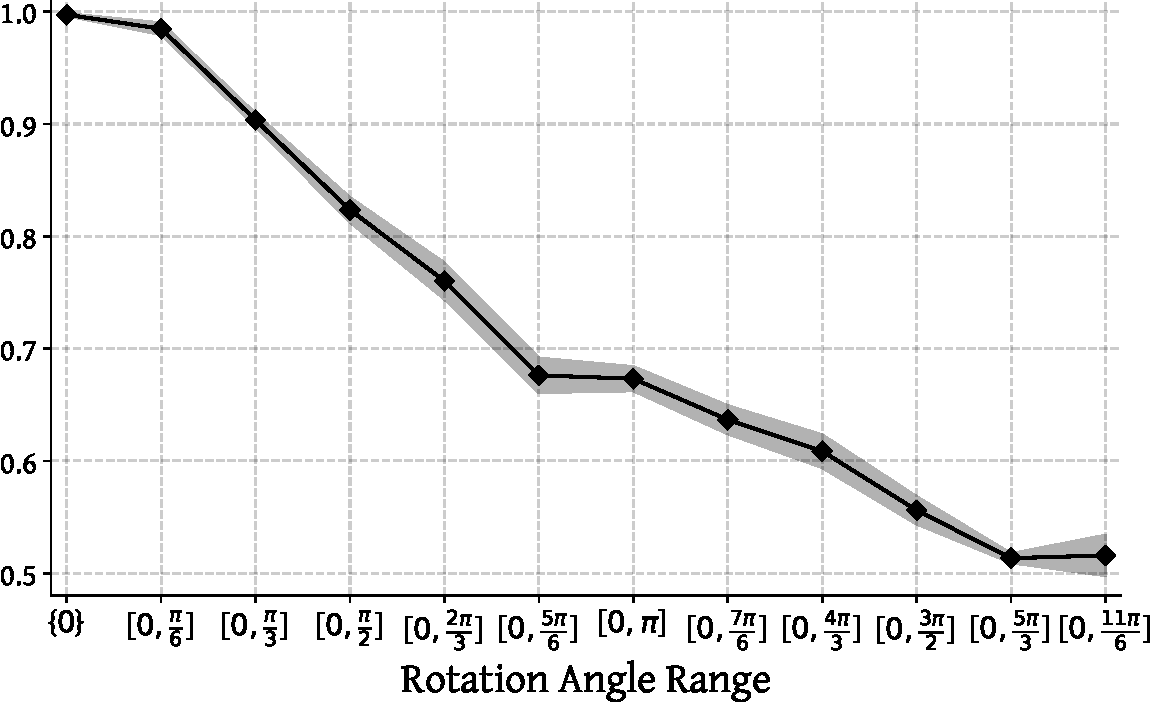
\includegraphics[width=\linewidth]{figs/eulearn/accuracy_vs_angle.pdf}
    \caption{\textbf{Classification accuracy of a $k$-nearest neighbor classifier vs. training rotation range.} Accuracy is perfect when training and testing on canonical orientations but collapses as random rotations along the z-axis are introduced, revealing orientation-dependent bias in EuLearn. \textit{Note:} Results are cross-validated with 5 folds.}
    \label{fig:eulearn-acc-angle}
\end{minipage}\hfill
\begin{minipage}{0.50\linewidth}
    \centering
    \begin{tabular}{c c c c}
        \toprule
        Training set & Test set & Training Acc. & Test Acc. \\
        \bottomrule
        \multirow{2}{*}{\raisebox{-0.9ex}{
\includegraphics[height=1em]{figs/utils/unrotated.pdf}}}
          & \raisebox{-0.9ex}{
\includegraphics[height=1em]{figs/utils/unrotated.pdf}}
          & \multirow{2}{*}{99.9} & $96.4_{\textcolor{red}{(-0.5)}}$ \\
          & \raisebox{-0.9ex}{
\includegraphics[height=1em]{figs/utils/rotated.pdf}}
          & & $16.3_{\textcolor{red}{(-83.6)}}$ \\
        \midrule
        \multirow{2}{*}{\raisebox{-0.9ex}{
\includegraphics[height=1em]{figs/utils/rotated.pdf}}}
          & \raisebox{-0.9ex}{
\includegraphics[height=1em]{figs/utils/rotated.pdf}}
          & \multirow{2}{*}{77.8} & $50.1_{\textcolor{red}{(-27.7)}}$ \\
          & \raisebox{-0.9ex}{
\includegraphics[height=1em]{figs/utils/unrotated.pdf}}
          & & $45.9_{\textcolor{red}{(-31.9)}}$ \\
        \bottomrule
    \end{tabular}
    \caption{\textbf{Linear probing accuracy on Point-BERT embeddings of canonical vs. rotated shapes.} Probes trained on canonical orientations (
\includegraphics[height=1em,valign=c]{figs/utils/unrotated.pdf}) achieve high accuracy only on canonical test data, collapsing under rotation. (
\includegraphics[height=1em,valign=c]{figs/utils/rotated.pdf}). Probes trained on rotated shapes generalize poorly in both cases, confirming that EuLearn does not provide a stable signal for genus.}
    \label{tab:eulearn-overfit}
\end{minipage}
\end{figure}

Taken together, these results demonstrate that EuLearn’s construction introduces systematic biases. The dataset does not allow disentangling true topological reasoning from pose-dependent shortcuts, making it unsuitable for evaluating structural understanding in 3D shape encoders.

\subsection{Sampling Labels}
\label{ssec:suppl_sampling_labels}

As mentioned in Section~\ref{sssec:labels-distribution}, labels (number of connected components $\beta_0$ and genus $g$) are sampled prior to generating any mesh. This step is key as it is where we ensure marginal distributions of both labels to be approximately uniform. The sampling procedure is described below. The algorithm takes as input the minimum and maximum number of connected components $\beta_0^{min}$ and $\beta_0^{max}$, the maximum genus per component $g^{max}$, the maximum genus per sample (group of components) $G^{max}$ and a parameter $k$ that controls the number of samples per value of $\beta_0$. It outputs a list of $(\beta_0, g)$ pairs, with $\beta_0\sim\mathcal{U}\llbracket \beta_0^{min}, \beta_0^{max} \rrbracket$ and $g\sim\mathcal{U}\llbracket 0, G^{max} \rrbracket$ subject to the constraint that $g \leq \min(G^{max}, \beta_0 \times g^{max})$. The constraint encodes that a single component can't have a genus higher than $g^{max}$, and that the total genus of a sample cannot exceed $G^{max}$. 

\paragraph{Role of $k$.} 
Choosing exactly $k$ times each value of $\beta_0$ ensures that the marginal distribution of $\beta_0$ is perfectly uniform. However, since the number of valid genus values depends on $\beta_0$, the marginal distribution of $g$ is only approximately uniform.


\begin{algorithm}
  \caption{Sampling $(\beta_0, g)$ \\ 
  \textbf{Input:} $g^{\max},\; G^{\max},\; \beta_0^{\min},\; \beta_0^{\max},\; k$} \label{alg:topogen-labels-sampling}

  \begin{algorithmic}[ ] % you can use [1] to turn on line numbering
    \State let $\mathfrak{B}_0 \gets \{\underbrace{\beta_0^{min}, \dots, \beta_0^{min}}_{\times k}, \underbrace{\beta_0^{min}+1}_{\times k}, \dots, \underbrace{\beta_0^{max}}_{\times k}\}$
    \State initialize output list $P \gets []$
    \ForAll{$\beta_0 \in \mathfrak{B}_0$}
      \State $g_{max} \gets \min\big(G^{max},\; \beta_0 \cdot g^{max}\big)$
      \State $\mathrm{accepted} \gets \mathrm{false}$
      \While{not $\mathrm{accepted}$}
        \State sample $s \sim \mathcal{U}\llbracket 0, G^{max} \rrbracket$
        \If{$s \le g_{\max}$}
          \State $\mathrm{accepted} \gets \mathrm{true}$
        \EndIf
      \EndWhile
      \State append $(\beta_0, s)$ to $P$
    \EndFor
    \Statex
    \Return $P$
  \end{algorithmic} 
\end{algorithm}

\begin{table}
\centering
\label{tab:topogen-hyperparams}
\begin{tabular}{l c}
\toprule
\textbf{Hyperparameter} & \textbf{Value} \\
\midrule
$g^{\max}$ & 5 \\
$G^{\max}$ & 10 \\
$\beta_0^{\min}$ & 1 \\
$\beta_0^{\max}$ & 6 \\
$k$ & 1000 \\
\bottomrule
\end{tabular}
\caption{Hyperparameter values used for the DONUT dataset for the experiments. Probing tasks boil down to classifying shapes across $\beta_0^{\max} - \beta_0^{\min} + 1 = 6$ categories for connected components and 11 categories for genera.}
\end{table}

\subsection{Choosing Components Shapes}
\label{ssec:suppl_choosing_components}

Once the labels are sampled, the next step is to choose the actual shapes composing each sample. This is done by decomposing the global genus $g$ into $\beta_0$ individual genera $(g_1, \dots, g_{\beta_0})$ such that $\sum_{i=1}^{\beta_0} g_i = g$. Each $g_i$ is then associated with a parametric family of shapes (Section~\ref{sssec:sample-level-properties}). However, given a couple $(\beta_0, g)$ several shapes configurations can lead to the same global labels (Figure ...). We leverage this observation to add more variability within the dataset, by first getting all the possible combinations of shapes for a given label configuration. The problem can be formulated as follows:

\begin{tcolorbox}[mybox]
  \textbf{Problem statement:} \emph{We're given three integers: $a$ (total items), $b$ (target weighted sum) and $g^{max}$ (maximum template index). We also have templates numbered from $0$ to $g^{max}$ (included). Template $i$ has a weight of $i$. \\ We want to find all the possible ways to distribute exactly $a$ items across these templates such that the weighted sum $\sum_{i=0}^{g^{max}} i \cdot x_i = b$, where $x_i$ is the number of items assigned to template $i$.} 

  \textbf{Input:}
  \begin{itemize}
    \item $a$: Total number of items to distribute
    \item $b$: Target weighted sum
    \item $g^{max}$: Maximum template index (templates are $0, 1, 2, \dots, g^{max}$)
  \end{itemize}

  \textbf{Output:} A list of all possible distributions $(x_0, x_1, \dots, x_{g^{max}})$.
\end{tcolorbox}

\begin{tcolorbox}[bluebox]
  \textbf{Example:}

  \textbf{Input:} $a = 3,\; b = 5,\; g^{max} = 3$

  \textbf{Output:} $\big[ [0, 2, 0, 1], [1, 0, 1, 1], [0, 1, 2, 0]\big]$

  \textbf{Explanation:}
  \begin{itemize}
    \item $[0, 2, 0, 1]$: $0 \cdot 0 + 2 \cdot 1 + 0 \cdot 2 + 1 \cdot 3 = 3$, and total count $0+2+0+1=3$
    \item $[1, 0, 1, 1]$: $1 \cdot 0 + 0 \cdot 1 + 1 \cdot 2 + 1 \cdot 3 = 5$, and total count $1+0+1+1=3$
    \item $[0, 1, 2, 0]$: $0 \cdot 0 + 1 \cdot 1 + 2 \cdot 2 + 0 \cdot 3 = 5$, and total count $0+1+2+0=3$
  \end{itemize}
\end{tcolorbox}

In the context of DONUT, $a$ corresponds to the number of connected components $\beta_0$, $b$ to the total genus $g$ and $g^{max}$ to the maximum genus per component. The output distributions $(x_0, x_1, \dots, x_{g^{max}})$ indicate how many components of each genus should be used to form a sample with the desired labels. For instance, if $\beta_0 = 3$, $g = 5$ and $g^{max} = 3$, one valid output is $(1, 0, 1, 1)$ which means that the sample should be composed of one genus-0 shape, zero genus-1 shapes, one genus-2 shape and one genus-3 shape. \textit{Note} that $G^{max}$ isn't directly involved here, as it's been used already to choose the values of $g$ (Algorithm \ref{alg:topogen-labels-sampling}).

\paragraph{Algorithmic Details.} 
Even though we seek for efficient algorithms to ensure the scalability of DONUT, finding all the combinations requires a tree search algorithm with backtracking. This procedure has exponential () complexity. However, since both $\beta_0^{max}$ and $G^{max}$ are small, enumerating all the solutions given $(\beta_0, g)$ requires a negligible amount of time compared to generating the actual meshes and composing them together. Once all the solutions are enumerated, we randomly sample one of them to generate the actual meshes. \textit{Note} that to avoid useless computations, we cache the solutions for each $(\beta_0, g)$ couple, so that if the same couple is encountered again, we can directly sample from the already computed solutions.

\paragraph{Complexity.}
A naïve approach of the algorithm's complexity is $O(a^{g^{max}+1})$, since at each of the $g^{max}+1$ recursion levels,  we can have up to $a$ branches. However, this bound is very loose, because the additional constraint on the weighted sum $b$ prunes most fo the branches: many partial assignments can't possbbly satisfy both the total count and the target sum, and are therefore discarded early. The algorithm actually enumerates \emph{weak combinations} \cite{counting} 

\begin{algorithm}
  \caption{\textsc{Enumerate-Solutions} \\
  \textbf{Input:} $a$, $b$, $g^{max}$ \\
  \textbf{Output:} $S$}
  \begin{algorithmic}[]
      \State $S \gets \emptyset$ \Comment{Initialize solution set}
      \If{$b < 0$ \textbf{ or } $b > g^{max} \cdot a$}
          \State \Return $S$
      \EndIf
      \State \Call{Backtrack}{$a, b, 0, \emptyset, S$} \Comment{Start recursive enumeration}
      \State \Return $S$
  \end{algorithmic}
\end{algorithm}

\begin{algorithm}
  \caption{\textsc{Backtrack} \\
  \textbf{Input:} $r_{\text{count}}$, $r_{\text{sum}}$, $k$, $\mathbf{x}$, $S$ \\
  \textbf{Output:} $S$}
  \begin{algorithmic}[]
      \If{$k > g_{\max}$} \Comment{Base case: all template types processed}
          \If{$r_{\text{count}} = 0$ \textbf{ and } $r_{\text{sum}} = 0$}
              \State $S \gets S \cup \{\mathbf{x}\}$
          \EndIf
          \State \Return
      \EndIf
      \Comment{Calculate upper bound for current template type}
      \If{$k = 0$}
          \State $u_k \gets r_{\text{count}}$
      \Else
          \State $u_k \gets \min(r_{\text{count}}, \lfloor r_{\text{sum}} / k \rfloor)$
      \EndIf
      \Comment{Try all feasible counts for template type $k$}
      \For{$n_k = 0$ \textbf{ to } $u_k$}
          \State $\mathbf{x}' \gets \mathbf{x} \cup \{n_k\}$
          \State \Call{Backtrack}{$r_{\text{count}} - n_k,\; r_{\text{sum}} - k \cdot n_k,\; k+1,\; \mathbf{x}',\; S$}
      \EndFor
  \end{algorithmic}
\end{algorithm}


\subsection{Baselines Training Details}
\label{ssec:topogen-baseline-training}

We provide here the training details for the baselines presented in Section~\ref{tab:topogen-results}.

\begin{table}[h!]
  \centering
  \begin{tabular}{l|ccc|ccc}
  \toprule
    & \multicolumn{3}{c|}{\textbf{Point-based models}} & \multicolumn{3}{c}{\textbf{Topology-based models}} \\
    Hyperparameter  & PointNet & PointNet++ & DGCNN & PersFormer & xPerT & PersLay \\
  \midrule
  Batch size              & 32    & 32    & 32    & 64    & --    & -- \\
  Learning rate           & 0.001 & 0.001 & 0.005 & 0.0005 & -- & -- \\
  Optimizer               & Adam  & Adam  & Adam  & AdamW  & --  & -- \\
  Weight decay            & 1e-4  & 1e-4  & 1e-4  & 5e-5  & --  & -- \\
  Dropout                 & 0.3   & 0.3   & 0.5   & 0.5   & --   & -- \\
  Training epochs         & 200   & 200   & 250   & 300   & --   & -- \\
  \bottomrule
  \end{tabular}
  \caption{Comparison of typical training hyperparameters for point-based models (PointNet, PointNet++, DGCNN) and topology-based models (PersFormer, xPerT, PersLay). A vertical line separates the two families of architectures.}
  \label{suppl:topogen-baseline-training}
\end{table}

\subsection{Additional Results}
\label{ssec:topogen-additional-results}

We complete the results provided in Table~\ref{tab:topogen-results} with per-class metrics for each baseline. 
